\section*{Exercice ??? -- Dérivation vectorielle}
\setcounter{exo}{0}


On note $\mathcal{B}_0=\base{x}{y}{z}$, $\mathcal{B}_1=\base{u}{v}{z}$, $\mathcal{B}_2=\base{w}{z_1}{u}$ et $\mathcal{B}_3=\base{x_1}{y_1}{z_1}$.
\begin{center}
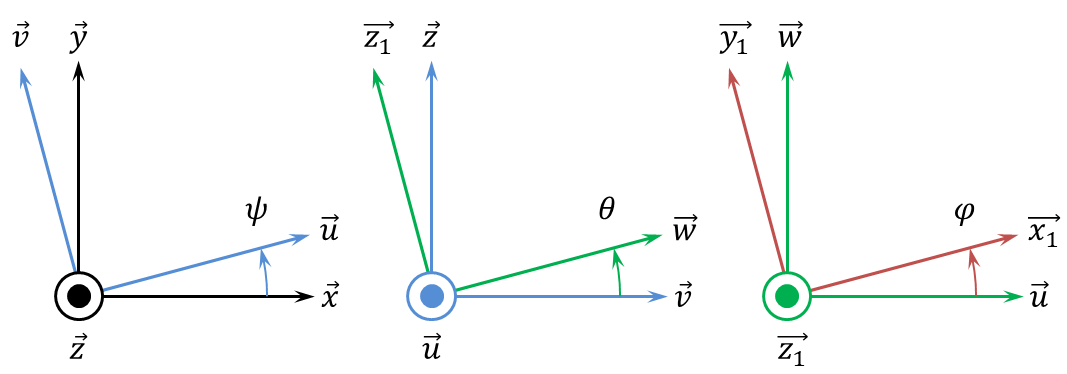
\includegraphics[width=\linewidth]{045_01}
\end{center}


\subparagraph{}
\textit{Donner la forumle de dérivation vectorielle.}

\subparagraph{}
\textit{Calculer les dérivées vectorielles suivantes (en exprimant le résultat dans la base la plus simple possible) : }
\begin{multicols}{3}
\begin{enumerate}
\item $\dfrac{\dd }{\dd t}\left[ \vect{x} \right]_{\mathcal{B}_0}$;
\item $\dfrac{\dd }{\dd t}\left[ \vect{u} \right]_{\mathcal{B}_0}$;
\item $\dfrac{\dd }{\dd t}\left[ \vect{v} \right]_{\mathcal{B}_0}$;
\item $\dfrac{\dd }{\dd t}\left[ \vect{w} \right]_{\mathcal{B}_0}$;
\item $\dfrac{\dd }{\dd t}\left[ \vect{z_1} \right]_{\mathcal{B}_0}$;
\item $\dfrac{\dd }{\dd t}\left[ \vect{x_1} \right]_{\mathcal{B}_0}$;
\item $\dfrac{\dd }{\dd t}\left[ \vect{y_1} \right]_{\mathcal{B}_0}$;
\item $\dfrac{\dd }{\dd t}\left[ \vect{x_1} \right]_{\mathcal{B}_1}$;
\item $\dfrac{\dd }{\dd t}\left[ \vect{y_1} \right]_{\mathcal{B}_1}$;

\end{enumerate}
\end{multicols}


